
\section{Dataset Description} \label{dataset-desc}

For the development and evaluation of the tracking system in this project, the CMU Panoptic Dataset \parencite{Joo_2015_ICCV,Joo_2017_TPAMI,Simon_2017_CVPR} has been used. This is a large-scale dataset that was originally recorded to facilitate research in multi-view social motion capture. \Cref{fig:examples} show a sample of some still images extracted from the video sequences contained in this dataset.

\begin{figure*}[ht!]
  \centering
  \begin{subfigure}[t]{\textwidth}
    \begin{subfigure}[t]{0.19\linewidth}
      \centering
      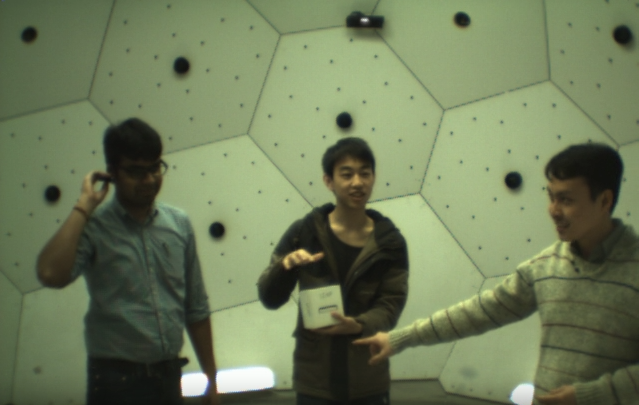
\includegraphics[width=\linewidth]{figures/examples/example1.png}
    \end{subfigure}
    \begin{subfigure}[t]{0.19\linewidth}
      \centering
      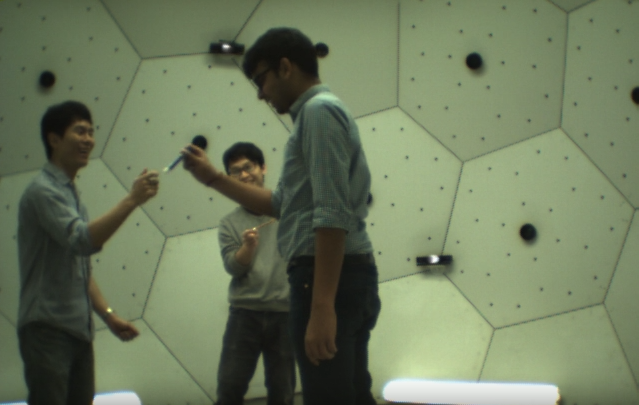
\includegraphics[width=\linewidth]{figures/examples/example2.png}
    \end{subfigure}
    \begin{subfigure}[t]{0.19\linewidth}
      \centering
      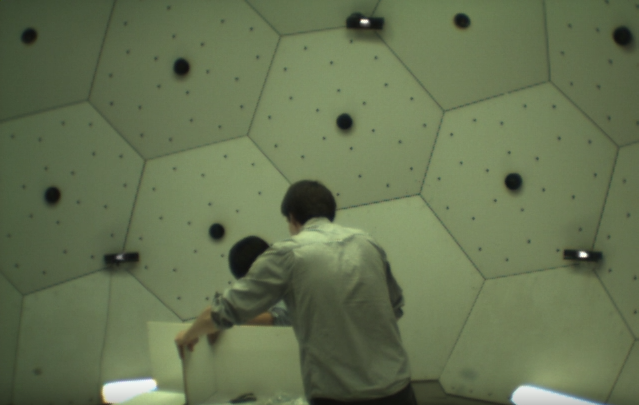
\includegraphics[width=\linewidth]{figures/examples/example3.png}
    \end{subfigure}
    \begin{subfigure}[t]{0.19\linewidth}
      \centering
      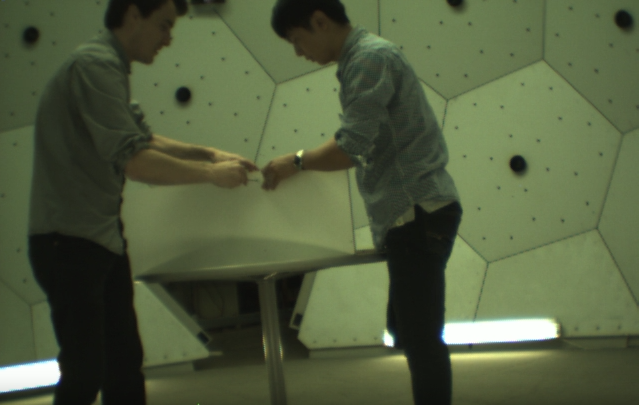
\includegraphics[width=\linewidth]{figures/examples/example4.png}
    \end{subfigure}
    \begin{subfigure}[t]{0.19\linewidth}
      \centering
      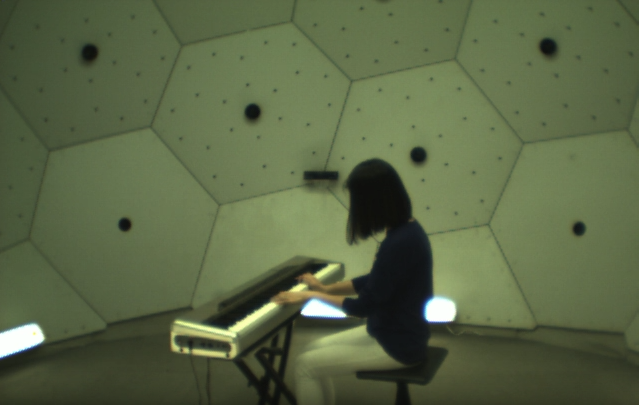
\includegraphics[width=\linewidth]{figures/examples/example5.png}
    \end{subfigure}
  \end{subfigure}
  \begin{subfigure}[t]{\textwidth}
    \begin{subfigure}[t]{0.19\linewidth}
      \centering
      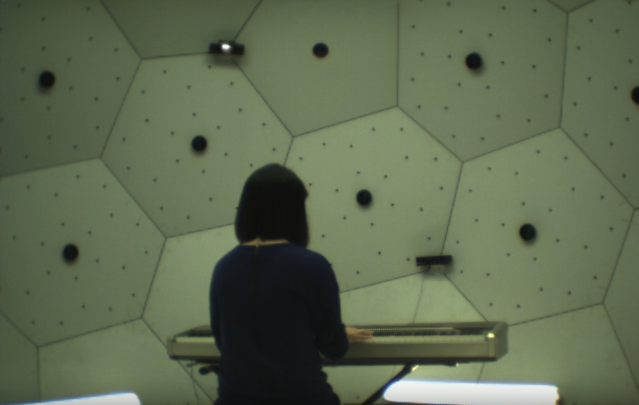
\includegraphics[width=\linewidth]{figures/examples/example6.png}
    \end{subfigure}
    \begin{subfigure}[t]{0.19\linewidth}
      \centering
      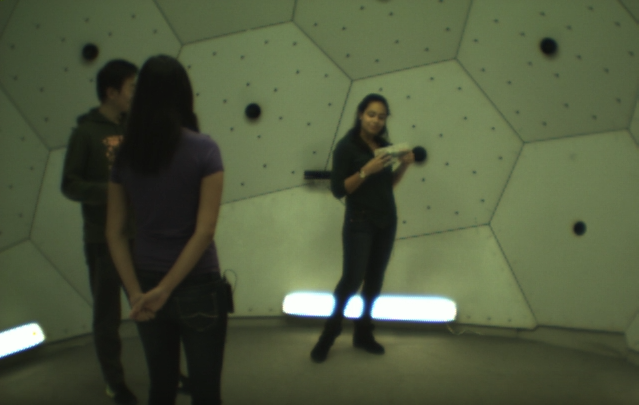
\includegraphics[width=\linewidth]{figures/examples/example7.png}
    \end{subfigure}
    \begin{subfigure}[t]{0.19\linewidth}
      \centering
      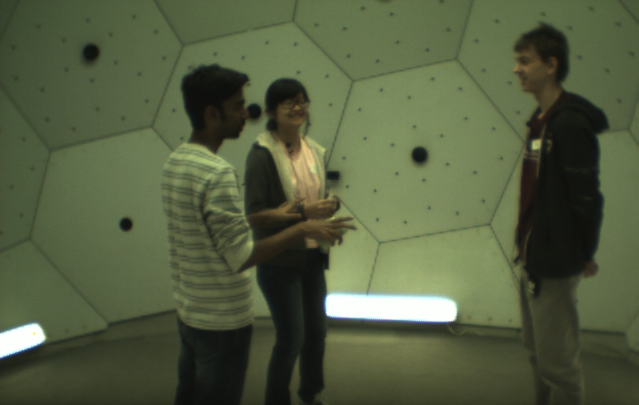
\includegraphics[width=\linewidth]{figures/examples/example8.png}
    \end{subfigure}
    \begin{subfigure}[t]{0.19\linewidth}
      \centering
      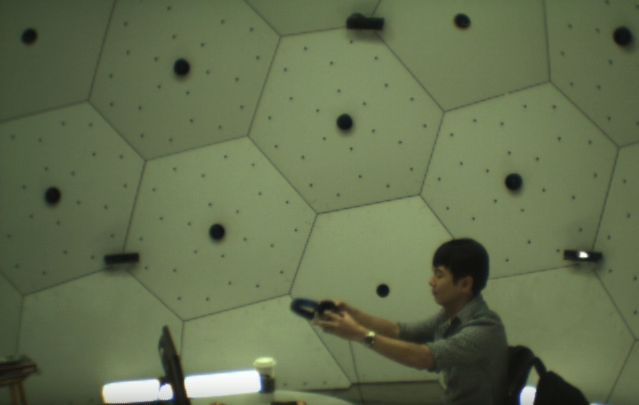
\includegraphics[width=\linewidth]{figures/examples/example9.png}
    \end{subfigure}
    \begin{subfigure}[t]{0.19\linewidth}
      \centering
      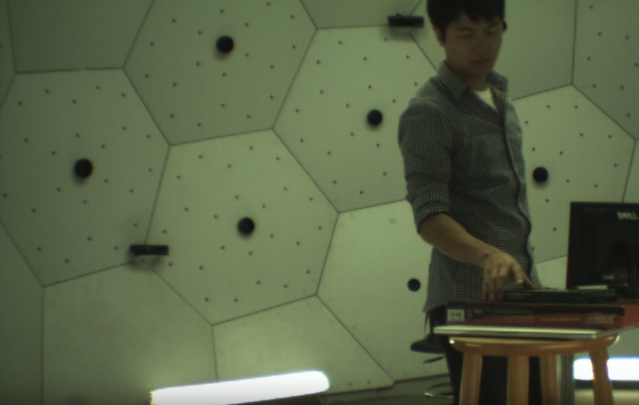
\includegraphics[width=\linewidth]{figures/examples/example10.png}
    \end{subfigure}
  \end{subfigure}
  \caption{A series of example images extracted from the video sequences of the CMU Panoptic dataset.}
  \label{fig:examples}
\end{figure*}

The complete dataset includes 84 video sequences totaling approximately 11.5 hours of video captured in a specialized 5.49m diameter dome-shaped room equipped with inward facing cameras attached to the outside panels. In total, the recording hardware consists of 511 calibrated cameras, 480 VGA cameras recording at a $640 \times 480$ resolution at 25 fps and 31 HD cameras recording at a $1920 \times 1080$ resolution at 30 fps. The room also contains 10 Kinect II \parencite{kurillo2022evaluating} sensors and 5 DLP projectors. Because of the geometry of the room and the placement of cameras, no single camera is able to view the complete space. This means that while each point in the space is visible from multiple cameras, each camera only captures a partial view of the environment, introducing occlusion and field-of-view limits related challenges for the tracking task.

The dataset also includes ground truth 3D skeletons and tracks that were generated by the CMU researchers using algorithms that leverage the entirety of the camera array \parencite{Joo_2015_ICCV}. Ground truth annotations of the dataset are provided in the COCO19 format. To align them with the outputs of the YOLO-based pose estimation networks used in this project \parencite{ultralyticsYOLO}, the ground truth data was pre-processes by converting it into the COCO17 format \parencite{lin2014microsoft}. This was achieved by discarding the two extra joint positions. The dataset also includes the calibration parameters for all available camera views, including camera extrinsics, intrinsics, and distortion parameters.

Due to computational and time constraints, running the tracking system across all the sequences for the dataset was not feasible. For this reason, a subset of the dataset was selected. Five video sequences were used for the evaluation, namely \inlinecode{171204_pose6}, \inlinecode{161029_piano4}, \inlinecode{170915_office1}, \inlinecode{161029_build1}, and \inlinecode{160224_haggling1}. Furthermore, evaluation was performed using only a subset of all camera views. A maximum of 16 VGA-type cameras were utilized per video sequence. These 16 cameras were selected based on the official dataset download script \footnote{\url{https://github.com/CMU-Perceptual-Computing-Lab/panoptic-toolbox/blob/master/scripts/getData.sh}}, which ensures they are approximately uniformly distributed around the dome to provide maximum spatial coverage with a minimal camera count.
